\documentclass[notes]{subfiles}

\begin{document}
	\addcontentsline{toc}{section}{5.2 - Volumes}
	\refstepcounter{section}
	\fancyhead[RO,LE]{\bfseries \large\nameref{cs52}} 
	\fancyhead[LO,RE]{\bfseries \currentname}
	\fancyfoot[C]{{}}
	\fancyfoot[RO,LE]{\large \thepage}	%Footer on Right \thepage is pagenumber
	\fancyfoot[LO,RE]{\large Chapter 5.2}
	
\section*{Volumes}\label{cs52}
	\subsection*{Before Class}
	\addcontentsline{toc}{subsection}{Before Class}
	\subsubsection*{Volumes by Cross-Sections}
	\addcontentsline{toc}{subsubsection}{Volumes by Cross-Sections}
		\begin{ex}
			An isosceles triangle has a base of 10 inches and height of 5 inches.  From geometry, we know that its area is 25 in$^2$; use integrals to find its area by slicing \emph{vertically}, then by slicing \emph{horizontally}.
		\end{ex}
			\vs{1}
		
		\begin{ex} 
		Describe how to find the volume of the triangular prism given below.  \\[5pt]
			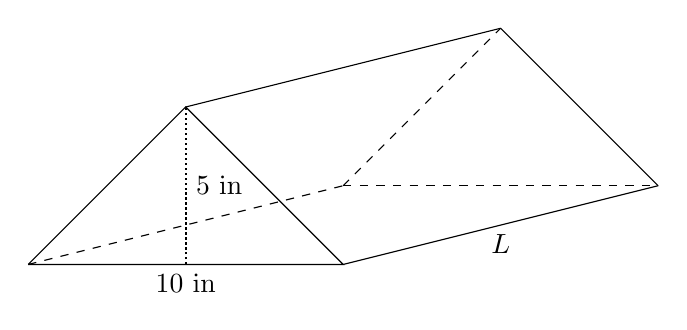
\begin{tikzpicture}
				\draw (0,0)--(2,2)--(4,0)--(0,0) node[midway, below] {10 in};
				\draw (6,3)--(8,1);
				\draw[dashed] (4,1)--(6,3);
				\draw[dashed] (4,1)--(8,1);
				\draw (2,2)--(6,3);
				\draw (4,0)--(8,1) node[midway, below] {$L$};
				\draw[dashed] (0,0)--(4,1);
				\draw[thick,densely dotted] (2,0)--(2,2) node[midway,right] {5 in};
			\end{tikzpicture}
		\end{ex}
			\vs{.25}
			\newpage
			
		\begin{ex}
			Show that the volume of a right cylinder of radius $r$ and height $h$ has volume $V = \pi r^2h$
		\end{ex}
			\vs{1}
		
		For generic volumes, we can consider cross sections of a solid, and ``slabs'' of constant width.
		\begin{defn}[Volume]
			Let $S$ be a solid that lies between $x =a $ and $x = b$.  If the cross-sectional area of $S$ in the plane $P_x$, through $x$ and perpendicular to the $x-$axis is $A(x)$, where $A$ is a continuous function, then the \textbf{volume} of $S$ is given by
			\showto{ins}{
				\[V = \lim_{n\to\infty} \sum_{i=1}^n A(x_i^*)\,\Delta x = \int_a^b A(x)\,dx\] 
			}
			\showto{st}{
				\vspace{.5in}
			}
		\end{defn}
		
		\begin{ex}
			Show that the volume of a sphere of radius $r$ is $V = \dfrac{4}{3}\pi r^3$
		\end{ex}
			\vs{1}
			\newpage
	\subsubsection*{Pre-Class Activities}
	\addcontentsline{toc}{subsubsection}{Pre-Class Activities}
		\begin{ex}
			Draw an explicit connection between how we found area under a curve in \S4.1 and \S4.2, and how we've defined area here.
		\end{ex}
			\vs{.25}
			
		\begin{ex}
			Use cross-sectional areas to prove that the volume of a square-based pyramid is $\dfrac{1}{3}L^2h$, where $L$ is the side length of the square base, and $h$ is the pyramid's height.
		\end{ex}
			\vs{1}
			
		\begin{ex}
			A wedge is cut out of a circular cylinder of radius 5 by two planes.  One plane is perpendicular to the axis of the cylinder.  The other intersects the first at an angle of $45\dc$ along a diameter of the cylinder.  Find the volume of the wedge.
		\end{ex}
			\vs{1}
			\newpage
			
	\subsection*{In-Class}
	\addcontentsline{toc}{subsection}{In-Class}
	\subsubsection*{Disk Method}
	\addcontentsline{toc}{subsubsection}{Disk Method}
		\begin{ex}
			Let $f(x) = 3$.
			\begin{enumerate}[(a)]
				\item Sketch the function on the interval $[0,2]$, and find the area between the curve and the $x-$axis on $[0,2]$.
					\vs{2}
				\item Sketch the cylinder created by rotating the line segment around the $x-$axis; what is the volume of the cylinder?
					\vs{1}
					
				\item Write an expression for a slice of the volume of the cylinder.
					\vs{1}
					\newpage
					
				\item Create and evaluate an integral expression for the volume of the cylinder.
					\vs{1}
			\end{enumerate}
		\end{ex}
			
		\begin{ex}
			Let $f(x) = 3x$
			\begin{enumerate}[(a)]
				\item Sketch the region bounded by $f(x)$, $x = 1$, and the $x-$axis.
					\vs{1}
					
				\item Sketch the solid created by rotating the region about the $x-$axis on $[0,1]$.
					\vs{1}
					
				\item Sketch and label an approximating cylinder for the volume of the cone.
					\vs{1}
					\newpage
					
				\item Create and evaluate an integral expression to find the volume of the cone.
					\vs{1}  
			\end{enumerate}
		\end{ex}
		

		\begin{rmk}[Disk Method]
			If $f$ is a positive, continuous function on some interval $[a,b]$, then the volume of the solid created by rotating $f(x)$ about the $x-$axis is given by
			\showto{ins}{
				\[\int_a^b \pi [r(x)]^2\, dx\]
			}
			\showto{st}{
				\vspace{.5in} \\
			}
			where $r(x)$ is the 
			\showto{ins}{
				\fbox{radius function}.
			}
			\showto{st}{
				\blank{2.5}.
			}
		\end{rmk}
		\begin{ex}
			Find the volume of the solid obtained by rotating the region under the curve $y = \sqrt{x}$ from 0 to 1, about the $x-$axis.  Sketch the region and a typical approximating cylinder.  
		\end{ex}
			\vs{1}

			\newpage
			
		\begin{ex}
			Find the volume of the solid obtained by rotating the first-quadrant region bounded by $y = x^2$, $y = 4$, and $x = 0$ about the $y-$axis.
		\end{ex}
			\vs{1}
			
		\begin{ex}
			Find the volume of the solid formed by revolving the region between the parabola $x = y^2 + 1$ and the line $x = 3$ about the line $x = 3$.
		\end{ex}	
			\vs{1}
			\newpage
			
	\subsubsection*{Washer Method}
	\addcontentsline{toc}{subsubsection}{Washer Method}
		\begin{ex}
			Let $f(x) = x^2$.
			\begin{enumerate}[(a)]
				\item Sketch the first-quadrant region bounded by $f(x)$ and the line $y = 4$.
					\vs{1}
						
				\item Sketch the solid resulting from rotating the region about the line $y = 0$.
					\vs{1}
					
				\item What are some problems with using the disk method in this example?
					\vs{1}
			\end{enumerate}
		\end{ex}
			\newpage
			
		\begin{ex}
			Find the volume of the solid formed by rotating the region bounded by $y = x^2$ and $y = x$ about the $x-$axis.  
		\end{ex}
			\vs{2}
		
		\begin{rmk}[Washer Method]
			If $f$ and $g$ are two continuous functions on $[a,b]$ such that $f(x) \geq g(x)$ on $[a,b]$, then the volume of the solid created by rotating the region between $f$ and $g$ is given by
			\showto{ins}{
				\[\int_a^b \pi\left[(R(x))^2- (r(x))^2\right]\, dx\]
			}
			\showto{st}{
				\vspace*{1in}\\
			}
			where $R(x)$ is the 
			\showto{ins}{
				\fbox{outer radius}
			}
			\showto{st}{
				\blank{3}
			}
			and $r(x)$ is the \\[20pt]
			\showto{ins}{
				\fbox{inner radius}.
			}
			\showto{st}{
				\blank{3}.
			}
		\end{rmk}
			\newpage
				
		\begin{ex}
			Find the volume of the solid obtained by rotating the region from the previous example about the line $y=1$.
		\end{ex}
			\vs{1}
			
		\begin{ex}
			The region bounded by the curve $y = x^2 + 1$ and the line $y = -x + 3$ is revolved about the $x-$axis to generate a solid.  Find the volume of the solid.
		\end{ex}	
			\vs{1}
			\newpage
		
		\begin{ex}
			Find the volume of the solid obtained by rotating the region bounded by the curves $y = x+1,y=0,x=0,x=2$ about the $x-$axis.
		\end{ex}
			\vs{1}
			
		\begin{ex}
			Find the volume of the solid obtained by rotating the region bounded by the curves $y = \sqrt{25-x^2},y=0,x=2,x=4$ about the $x-$axis.
		\end{ex}
			\vs{1}
			\newpage
				
	\subsection*{After Class}	
	\addcontentsline{toc}{subsection}{After Class}		
		\begin{ex}
			Find the volume of the solid obtained by rotating the region bounded by the curves $y = 2\sqrt{x}, y=2, x=0$ about the $x-$axis.
		\end{ex}
			\vs{1}
			
		\begin{ex}
			Find the volume of the solid obtained by rotating the region bounded by the curves $y = x^2,x=y^2$ about $y = 1$.
		\end{ex}
			\vs{1}
			\newpage
			
		\begin{ex}
			Find the volume of the solid created by rotating the the region bounded by the curves $y= x^3$, $y = 0$, and $x = 1$ about $x = 2$.
		\end{ex}
			\vs{1}
			
	\clearpage
\end{document}